\chapter{Introduction to Auto-Scaling}
\label{intro-auto-scale}

\section{Introduction}
\label{ias:intro}

As mentioned in Chapter~\ref{prob-def} the key characteristic of cloud environments is emph{elasticity} behavior. However, manually adjusting resources are is not effective approach to exploit this feature. Hence, we need to automate this procedure with minimal human intervention. This chapter introduces foundations of Auto-Scaling techniques. Different techniques and architectures will be discussed from a high level standing point. It shall be noted that, this chapter has been heavily inspired by work done by~\textcite{Lorido-Botran2014}.

\section{Basic Concepts}
\label{ias:basics}

The ultimate goal of an Auto-Scaling system is to automate the process of acquiring and releasing \emph{resources} in order to minimize the \emph{cost} with minimum violation of \emph{service level objectives} (SLO). However, \emph{resource} is a broad and context-dependent term. It refers to any form processing engine that provides application developers some form of computation power. This general purpose definition is broad enough to capture different kinds. In most cases it, it means virtual machines allocated by cloud provider. In more modern distributed systems, a resource refers to \emph{container}s like Google Kubernetes~\cite{kuber}. However, a resource might be as simple as a single process or thread.

The term \emph{cost} refers to any form of expenditure that users pay in order to acquire a resource. It doesn't necessarily mean \emph{monetary} cost. It can also refer to numerical values of resources, like number of virtual machines or number of running processes. Although minimizing cost is the ultimate goal of any Auto-Scaler system, not in all cases cost reduction is desirable. It should be achieved with respect to defined \emph{service level objectives}.

\emph{Service Level Objective}s are any predefined rules that shall be respected during application runtime. The following, defines a couple of SLO definitions for different applications:
\begin{itemize}
    \item 99 percentile round-trip latency of requests in a web application should be less than 150 milliseconds.
    \item All committed records in master database must be replicated with a maximum delay of 5 milliseconds.
    \item All messages pushed by a producer, should be processed by respective consumers in less than 5 minutes.
    \item At least 95\% of images published in the last 24 hours should be served by cache servers.
\end{itemize}
Service Level Objectives are typically determined and defined by business requirements. Defining effective and meaningful SLOs is a challenge on its own. However, it is out of the scope of this thesis.

To make an effective decision, an Auto-Scaler needs to consider application and its environment:
\begin{itemize}
    \item \textbf{Infrastructure pricing model}. Some infrastructure providers charge customers hourly. That is, if customer acquires a resource at 10:30AM and releases it at 11:30AM, the customer is charged for two hours. Some other service providers might charge on minute basis. Pricing model has a huge impact on decisions made by Auto-Scaler system, since it makes some decisions pointless.
    \item \textbf{Service level objectives}. Each application has its own set of objectives that should be adhered by Auto-Scaling system. These SLOs might be defined and applied at \emph{soft} and \emph{hard} levels. Violating an SLO at soft level is not critical, albeit alarming. However, violating a resource at hard level is a critical issue and is a negative point for an Auto-Scaler.
    \item \textbf{Acquire/Release delay}. Depending on type of the resource, it might take some time for the resource to become responsive and ready to process user requests. For example, booting a virtual machine typically takes couple of minutes, whereas launching a container takes time in order of seconds. An Auto-Scaler shall consider whether acquiring and releasing a heavy weight resource in a \emph{zig-zag} manner worth the overhead or not.
    \item \textbf{Unit of allocation}. In some cases, it might be beneficial to allocate multiple instances of a same resource at once. This might be due to the startup and initialization overhead or it might be the case that Auto-Scaler predicted a huge load spike in near future.
\end{itemize}

Auto-Scaling can be done with different techniques and strategies. The remainder of this chapter is organized as follows. Section~\ref{ias:arch} defines general architecture of an Auto-Scaler. Section~\ref{ias:actions} clarifies which sort of actions can be applied by an Auto-Scaler. Section~\ref{ias:taxonomy} classifies different techniques and briefly explains each category. Finally, section~\ref{ias:conc} concludes.

\section{Auto-Scaler Architecture}
\label{ias:arch}

Figure~\ref{fig:auto-scaler-arch} illustrates generic architecture of an Auto-Scaler. This architecture is broad enough to capture different kinds of applications.
\begin{figure}[h]
    \centering
    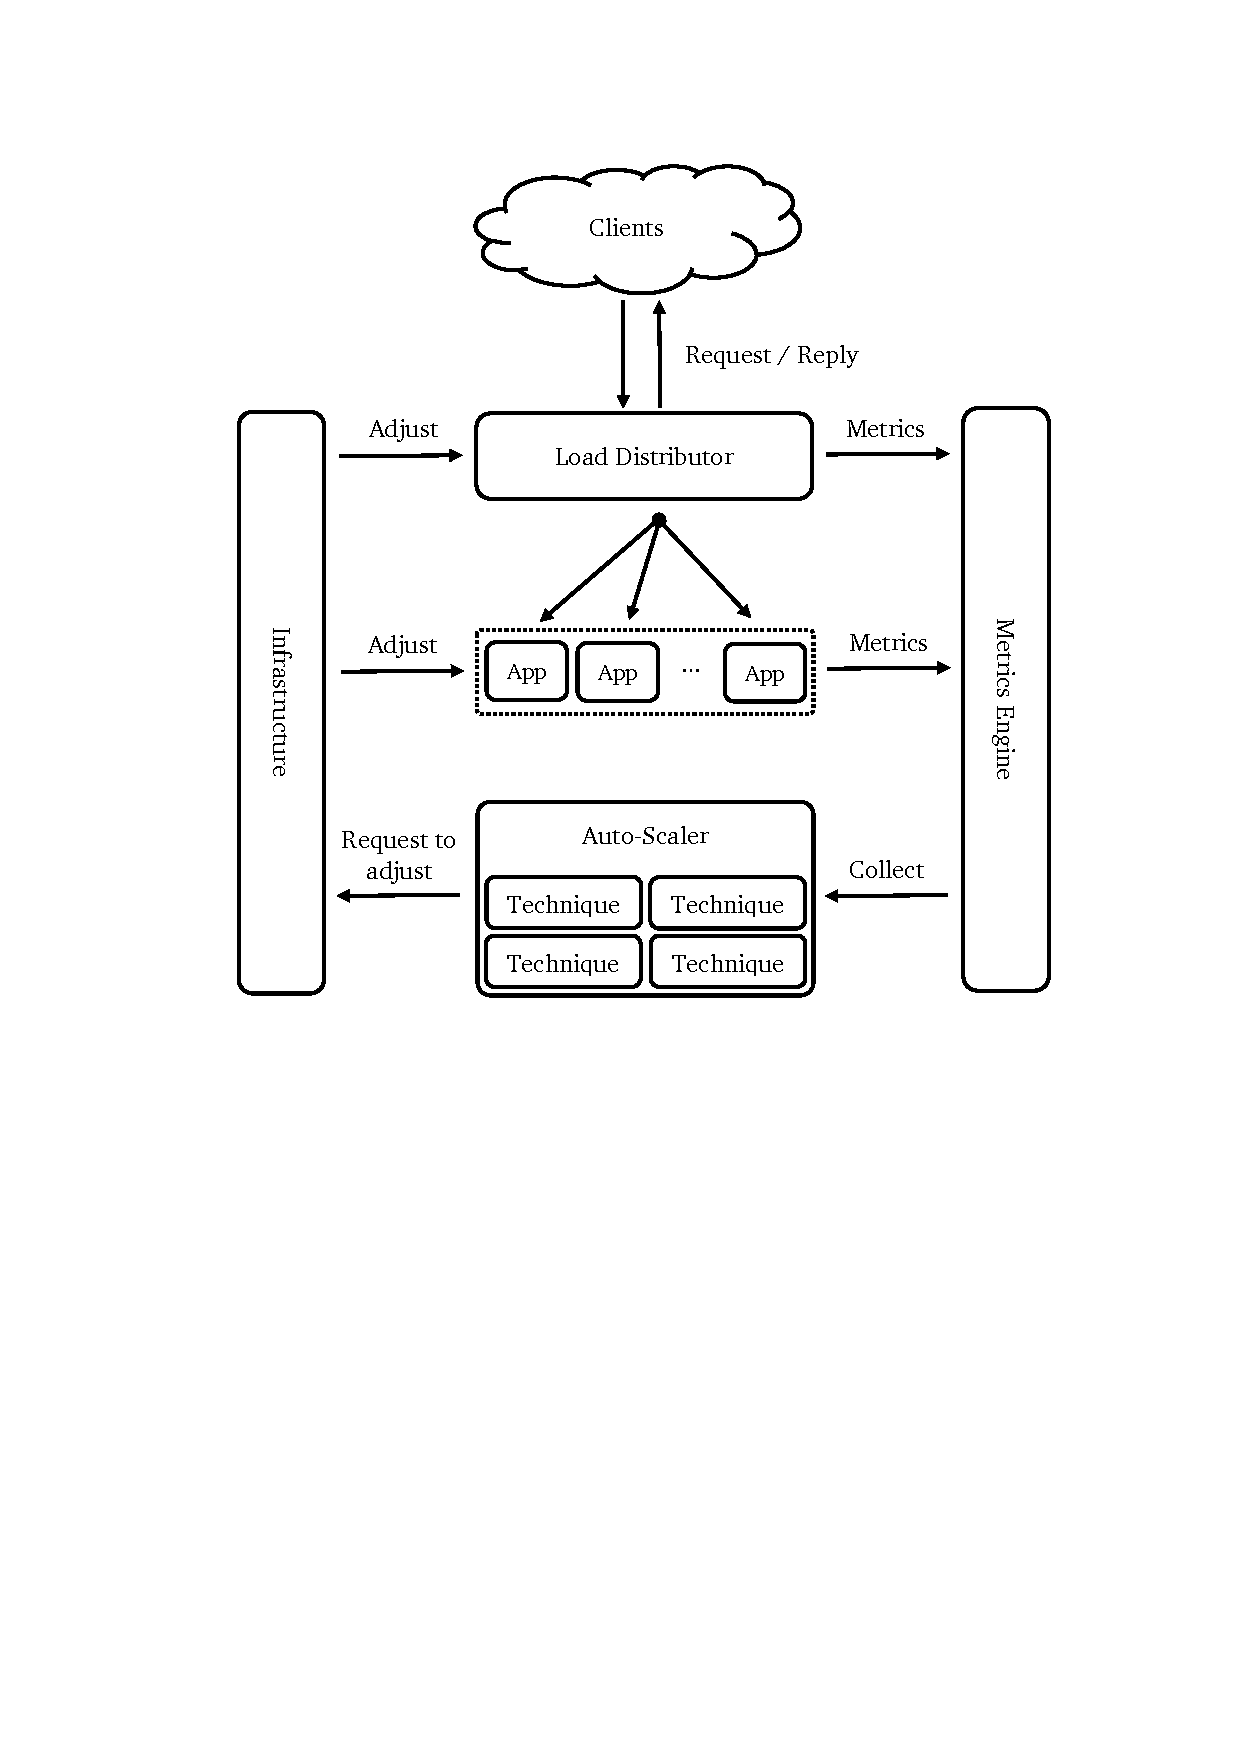
\includegraphics[clip, trim=3cm 12.5cm 2.5cm 2.5cm]{auto-scaler-arch.pdf}
    \caption{General Auto-Scaler Architecture}
    \label{fig:auto-scaler-arch}
\end{figure}
First, responsibilities of different components shall be clarified. Table~\ref{tab:auto-scaler-sum} summarizes all components of the system.
\begin{table*}
    \begin{tabular}{ll}
        \toprule
        \textbf{Component} & \textbf{Description}\\
        \midrule
        Clients & Users of the application which might be applications on their own\\
        Load Distributor & Distributes incoming requests to application instances\\
        Application & Runs business logic defined by developer\\
        Metric Engine & Monitors and collects metric from application and provides it to other components\\
        Infrastructure API & Provides API to adjust (add/remove) resources\\
        Auto-Scaler & Runs the auto-scaling algorithm based on metric collected by Metric Engine\\
        \bottomrule
    \end{tabular}
    \centering
    \caption{Auto-Scaler components summary}
    \label{tab:auto-scaler-sum}
\end{table*}
An Auto-Scaling system typically consists of following sub-components.
\begin{description}[leftmargin=0pt]
    \item[Clients] Most kinds of applications, typically have some form of client that sends requests to the system and either waits to get a reply or operates under \emph{fire-and-forget} strategy. It shall be noted that, a client is not necessarily an end user. In today's modern distributed applications, an application might be client of another application.
    \item[Load Distributor] In order to provide some degree of \emph{transparency}, usually clients connect to a Load Distributor component. It is the responsibility of the Load Distributer that \emph{proxies} client request to application. Load Distributor is also a generic component and might represent different technology in read-world applications. In the context of a web application, it might be an HTTP load balancer. Even a \emph{Message Broker} can also be represented as a form of Load Distributer. It shall be noted that Load Distributor itself can be replicated or sharded for \emph{high availability} or \emph{scalability} reasons.
    \item[Application] The application component runs the business logic. This architecture doesn't impose any limitation on application architecture. It might be a simple stateless web application. It might access to a back-end cache or database service. It might push some messages to a message broker, as a result of client request. It might be just a simple process consuming messaging provided by a message broker. It might forward client requests to other applications for further processing.
    \item[Metric Engine] Auto-Scaler system needs to have a good insight on current status of the application and incoming requests. Metric engine -- known as \emph{monitoring engine} takes the responsibility of measuring and collecting different aspects of the application. The term \emph{metric} refers to any form of measurable aspect of an application or its environment. \textcite{Ghanbari:2011} has defined and proposed a list of different type of metrics that could be exploited for different purposes.
    \begin{itemize}
        \item \textbf{Hardware} dependent metrics such as CPU usage, disk access time, memory usage, network bandwidth usage, network latency.
        \item \textbf{Operating System} provided metrics such as CPU-time, page faults, real memory.
        \item \textbf{Load balancer} provided metrics such as size of request queue length, session rate, number of current sessions, transmitted bytes, number of denied, requests, number of errors.
        \item \textbf{Web server} provided metrics such as transmitted bytes and requests, number of connections in specific states (e.g. closing, sending, waiting, starting, \dots).
        \item \textbf{Application server} provided metrics such as total threads count, active threads count, used memory, session count, processed requests, pending requests, dropped requests, response time.
        \item \textbf{Database server} provided metrics such as number of active threads, number of transactions in a particular state (e.g. write, commit, roll-back, \dots).
    \end{itemize}
    Since storing and reporting metrics has its own overhead, typically metrics engine aggregates collected values at different scale depending on how fresh it is. Rationally, fresh values are more important for Auto-Scaling system. As an example, it might provide near real time values for about 15 minutes. Then, for the last 5 hours, collected values are aggregated by a window of one minute. For last two days, it is aggregated by a window of 15 minutes and finally, for any record older than last two days, it is aggregated on hourly basis. Whether these aggregated values are sufficient for Auto-Scaler to make an accurate decision is out of the scope of this thesis. However, it may be a good idea to empirically adjust this system until it fits the requirements of Auto-Scaler system.
    \item[Infrastructure API] Typically, when an Auto-Scaler system decides to take any action, it doesn't touch the application directly. In order to provide \emph{separation of concerns}, this responsibility is handed over to infrastructure via an API provided by resource/service provider. An important issue that shall be noted here is that, service provider may schedule resource changes and execute them some time later. Thus, resource changes might not take effect immediately at the moment Auto-Scaler requests them. This fact shall be considered by Auto-Scaler system.
    \item[Auto-Scaler] This component is the core of Auto-Scaling system. It consists of different techniques. Typically, an Auto-Scaler works in \emph{consecutive rounds}. First, it collects metrics from Metrics Engine and offloads them to one or multiple technique implementations. It shall be noted that, an Auto-Scaler might utilize different implementation of techniques simultaneously -- for different stages of the application as an example. Even it might utilize a single implementation under different configurations. This architecture does not impose any limit on the order of techniques. Then, based on some preferences or ordering mechanism, it chooses the \emph{final decision}. Finally, it requests the Infrastructure API to change the number of resources. Naturally the assumption is that, infrastructure provider should be able to adjust the required or released resources. However, in some case it might not be able to fulfill the task. Thus, Auto-Scaler shall wait for a response to check whether the request has been successfully fulfilled or not. 
\end{description}
For the sake of understandability, Algorithm~\ref{a:as-workflow} describes the above procedure in pseudo code.
\begin{algorithm}[h]
    \DontPrintSemicolon
    
    \SetKwFunction{GCMFME}{GetCurrentMetricsFromMetricsEngine}
    \SetKwFunction{GD}{GetDecision}
    \SetKwFunction{GFD}{GetFinalDecision}
    \SetKwFunction{RIA}{RequestInfrastructureAPI}
    \SetKwFunction{error}{LogError}
    \SetKwFunction{factory}{InstantiateTechnique}
    
    \SetKwArray{impls}{implementations}
    \SetKwData{impl}{impl}
    \SetKwArray{dec}{decisions}
    \SetKwData{finaldec}{finalDecision}
    \SetKwData{reply}{reply}
    
    \tcp{different implementations of techniques}
    \impls $\gets$ [] \;
    \tcp{decision of each implementation}
    \dec $\gets$ [] \;
    \tcp{final decision of Auto-Scaler}
    \finaldec $\gets$ null\;
    \;
    \tcp{instantiate as many techniques as required}
    \For{$i \gets 0$ \KwTo $n$}{
        \impls{i} $\gets$ \factory{i}
    }
    \;
    \Repeat{\textup{Auto-Scaler is running}} {
        \tcp{load monitoring data from metrics engine}
        currentMetrics $\gets$ \GCMFME{} \;
        \;
        \tcp{initialize decisions}
        \dec $\gets$ [] \;
        \For{$i \gets 0$ \KwTo $n$}{
            \impl $\gets$ \impls{i} \;
            \dec{i} $\gets$ \GD{\impl}
        }
        \;
        \tcp{calculate final decision based on some weight or ordering mechanism}
        \finaldec $\gets$ \GFD{\dec} \;
        \;
        \tcp{request infrstructure API to adjust resources}
        \reply $\gets$ \RIA{\finaldec}\;
        \;
        \tcp{in case infrastructure reject request, warn developers}
        \If{\reply = ReplyStatus.REJECT}{
            \tcp{issue a warning}
            \error{"request can not be fulfilled"}
        }
    }
    \caption{General workflow of an Auto-Scaler}
    \label{a:as-workflow}
\end{algorithm}
 
todo: write actions
todo: action horizental vs vertical
todo: strategy --> expoential allocations, ...
todo: pseoducode, gracen period
todo: trade off of meeting slo and costs

\section{Actions}
\label{ias:actions}

\section{Taxonomy of Auto-Scaling Techniques}
\label{ias:taxonomy}

\section{Conclusion}
\label{ias:conc}